\begin{enumerate}[label=\thesection.\arabic*,ref=\thesection.\theenumi]
\numberwithin{equation}{enumi}
\numberwithin{figure}{enumi}
\numberwithin{table}{enumi}

\item 
\item 
\label{chapters/11/11/5/2}
\iffalse

\documentclass[journal,10pt,twocolumn]{article}
\usepackage{graphicx}
\usepackage[margin=0.5in]{geometry}
\usepackage[cmex10]{amsmath}
\usepackage{array}
\usepackage{booktabs}
\usepackage{mathtools}
\usepackage{amssymb}
\title{\textbf{Conics Assignment}}
\author{lakshmi kamakshi}
\date{September 2022}
\providecommand{\norm}[1]{\left\lVert#1\right\rVert}
\providecommand{\abs}[1]{\left\vert#1\right\vert}
\let\vec\mathbf
\newcommand{\myvec}[1]{\ensuremath{\begin{pmatrix}#1\end{pmatrix}}}
\newcommand{\mydet}[1]{\ensuremath{\begin{vmatrix}#1\end{vmatrix}}}
\providecommand{\brak}[1]{\ensuremath{\left(#1\right)}}

\begin{document}

\maketitle
\paragraph{\textit{Problem Statement} -
\fi
\\
\solution
	\begin{figure}[!ht]
		\centering
 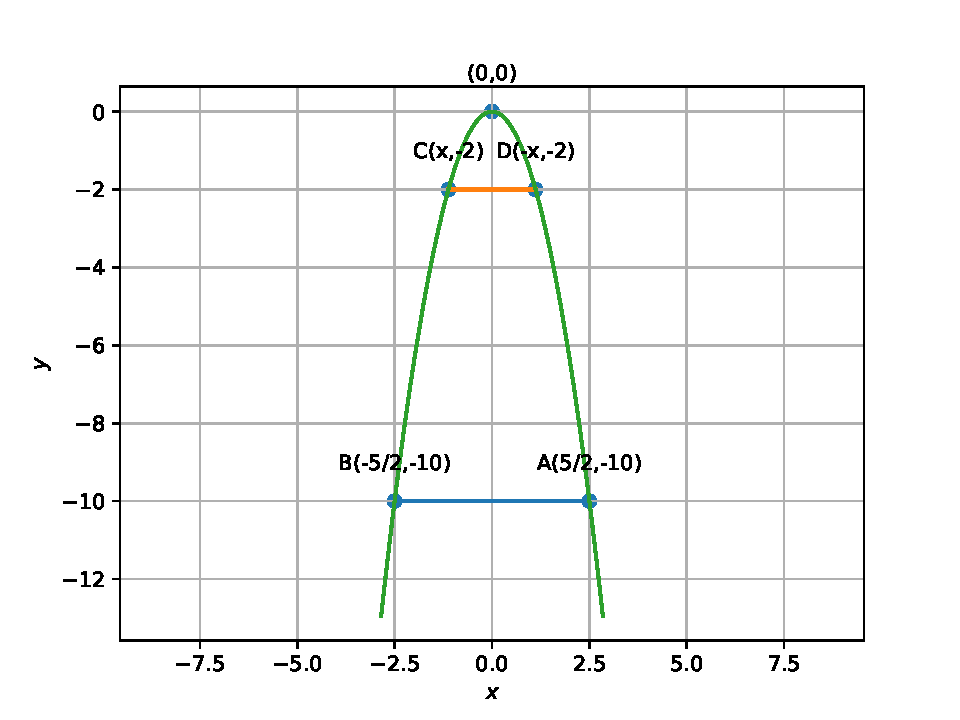
\includegraphics[width=\columnwidth]{chapters/11/11/5/2/figs/fig.pdf}
		\caption{}
		\label{fig:11/11/5/2}
  	\end{figure}
	\iffalse
} \vspace{5mm}

\section*{\large Solution}


Given, the axis of parabola is vertical,
\\ Let the equation of the axis be y-axis:
\begin{equation}
	\label{eq:parabola_q}
	\myvec{1\\0}\textbf{x}= 0
\end{equation}
\\ The above quadratic equation can be written in the general quadratic form as:

\begin{figure}[h]
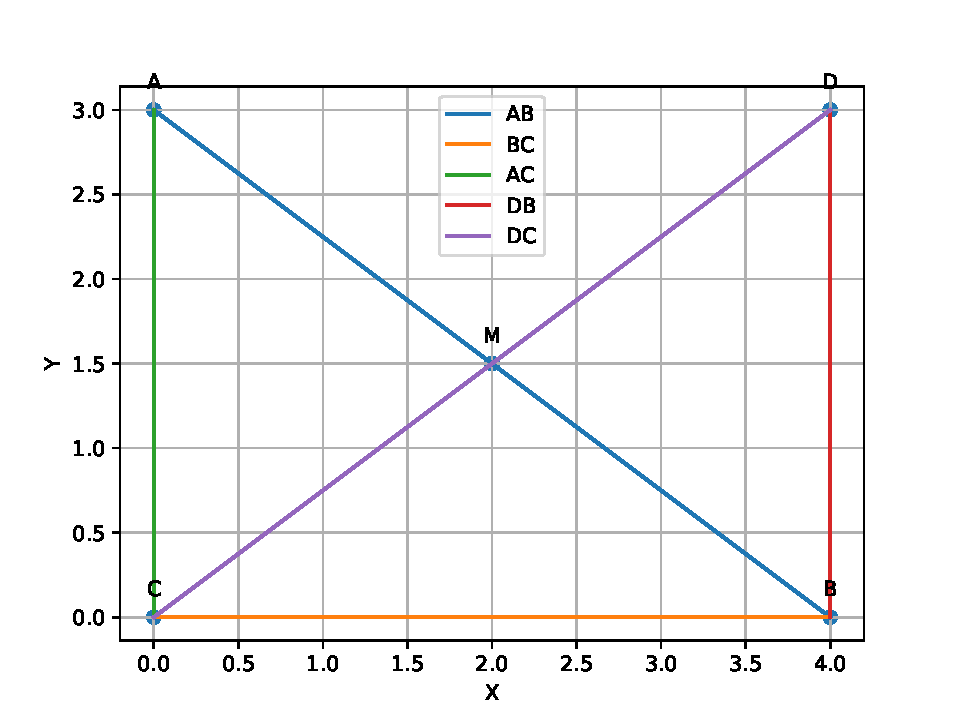
\includegraphics[width=0.8\columnwidth]{fig.pdf}
\end{figure}
\begin{equation}
	\label{eq:std_parabola}
	\textbf{x}^T\textbf{V}\textbf{x}+2\textbf{u}^T\textbf{x}+f=0
\end{equation}
where,
\begin{eqnarray}
\label{eq:Vec_V}
V = \myvec{1&0\\0&0}
\label{eq:Vec_U}
\\ u=\myvec{0\\2a}
\end{eqnarray}
\begin{equation}
\\ f =0
\end{equation}
Given arch is 10m high and 5m wide at the base. So the point $(\frac{5}{2},-10)$ lies on the parabola
\begin{equation}
	\myvec{X_1} = \myvec{\frac{5}{2}\\-10}
\end{equation}
\\ Substitute the point $X_1$ \\
\begin{eqnarray}
	\myvec{X_1}^T \myvec{V} \myvec{X_1} +2\myvec{u^T} \myvec{X_1} = 0
\\	a = \frac{5}{32}
\end{eqnarray}
\\Now , the matrix u will be,
\begin{equation}
	\myvec{u} = \myvec{0\\\frac{5}{16}}
\end{equation}
\\We need to find the width of parabola at a height of $2m$ from the vertex.So,the line parallel to x axis and passing through point $(0,-2)$ intersects the conic at 2 places C and D.
\\The line parallel to x-axis and passing through point $(0,-2)$ is
\begin{align}
	\myvec{X}\myvec{0\\1}^T = \myvec{2}
\end{align}
The points of intersection of the line 
\begin{align}
	L: \quad \vec{x} = \vec{q} + \mu \vec{m} \quad \mu \in \mathbf{R}
\label{eq:conic_tangent}
\end{align}
with the conic section  are given by
\begin{align}
\vec{x}_i = \vec{q} + \mu_i \vec{m}
\label{eq:conic_tangent_pts}
\end{align}
where 
{\tiny
\begin{multline}
\mu_i = \frac{1}
{
\vec{m}^T\vec{V}\vec{m}
}
\lbrak{-\vec{m}^T\brak{\vec{V}\vec{q}+\vec{u}}}
\\
\pm
\rbrak{\sqrt{
\sbrak{
\vec{m}^T\brak{\vec{V}\vec{q}+\vec{u}}
}^2
-
\brak
{
\vec{q}^T\vec{V}\vec{q} + 2\vec{u}^T\vec{q} +f
}
\brak{\vec{m}^T\vec{V}\vec{m}}
	}}
\label{eq:tangent_roots}
\end{multline}
}
\\
Substituting the line in the conic
\begin{align}
\brak{\vec{q} + \mu \vec{m}}^T\vec{V}\brak{\vec{q} + \mu \vec{m}}  
\\
+ 2 \vec{u}^T\brak{\vec{q} + \mu \vec{m}}+f &= 0
\\
\implies \mu^2\vec{m}^T\vec{V}\vec{m} + 2 \mu\vec{m}^T\brak{\vec{V}\vec{q}+\vec{u}} 
\\
+ \vec{q}^T\vec{V}\vec{q} + 2\vec{u}^T\vec{q} +f &= 0
\label{eq:conic_intercept}
\end{align}
Solving the above quadratic equations yeilds the roots.Let the point of intersections of line and curve be C and D.
\begin{align}
	C = q+ \mu_1m
	\\ D = q+ \mu_2m
\end{align}
\\The line CD will be
\begin{align}
	C-D = m(\mu_1-\mu_2)
	 \\ \textbf{m} = \myvec{1\\0}
\end{align}
The required width of parabola is the norm of the line CD.
\begin{align}
	||\boldsymbol{C-D}|| =
	2\sqrt{
\sbrak{
\vec{m}^T\brak{\vec{V}\vec{q}+\vec{u}}
}^2
-
\brak
{
\vec{q}^T\vec{V}\vec{q} + 2\vec{u}^T\vec{q} +f
}}
\end{align}
substitute the values of \vec{m},\vec{q},\vec{V} and \vec{u}
\begin{align}
	\frac{1}{2}||\vec{C-D}||^2 =
	\myvec{1&0}\brak{\vec{V}\myvec{0\\-2}+\vec{u}}\brak{\vec{V}\myvec{0\\-2}+\vec{u}}^T-
\end{align}
\begin{align*}
\brak
{
	\myvec{0&-2}\vec{V}\myvec{0\\-2} + 2\vec{u}^T\myvec{0\\-2} 
}
\end{align*}
 \begin{multiline}
	 \implies \sbrak{\myvec{1&0}\brak{\myvec{1&0\\0&0}\myvec{0\\-2} + \myvec{0\\\frac{5}{16}}}} \brak{\myvec{1&0\\0&0}\myvec{0\\-2} + \myvec{0\\\frac{5}{16}}}}^T  - \\
	 \\ \brak{\myvec{0&-2}\myvec{1&0\\0&0}\myvec{0\\-2} + 2\myvec{0 & \frac{5}{16}}\myvec{0\\-2} - 0} \\ \brak{\myvec{1&0}\myvec{1&0\\0&0}\myvec{1\\0}}
\end{multline}
\begin{align}
	\implies \sbrak{\myvec{1&0}\myvec{0\\\frac{5}{16}}}^2 - \brak{\myvec{0\\0}+2\myvec{0\\\frac{5}{-8}} - 0}(1) \\
 & = \myvec{5\\2}
\end{align}
\\The width of the Parabola at $2m$ height is the length of the line CD.  \begin{align} ||\vec{C-D}|| = \myvec{\sqrt{5}}$m$ \end{align} \section*{\large Construction} The input parameters are V,u,$X_1$,$y_2$ \\
\setlength\extrarowheight{7pt}
\begin{tabular}{|c|c|c|}
	\hline
	\textbf{Symbol}&\textbf{Value}&\textbf{Description}\\
	\hline
	$X_1$=\myvec{x_1\\y_1} & \myvec{\frac{5}{2}\\-10}&point at base \\[8pt]
	\hline
	$y_2$ & -2& height of point C\\[8pt]
	\hline
	$\vec{P}$&\myvec{0&1\\1&0}&eigenvectors of $\vec{V}$\\[8pt]
	\hline
	$\vec{c}$&$\myvec{0\\0}$&center of parabola\\
	\hline
	$\eta$&$\vec{u}^{\top}\vec{p}_1$&from Eq11\\[8pt]
	\hline
	$\lambda_2$&$\vec{e}_2^{\top}D\vec{e}_2$&from Eq9 \\[8pt]
	\hline
	$(\vec{A},\vec{B})$&\myvec{x_1&-x_1\\y_1&y_1}&points at the base\\[8pt]
	\hline
	$(\vec{C},\vec{D})$&\myvec{\sqrt{\frac{5y_2}{8}}&\sqrt{\frac{-5y_2}{8}}\\2&2}&points at 2m height\\[8pt]	\hline
\end{tabular}
\end{document}
\fi

\item 
\item 
\label{chapters/11/11/5/4}
\iffalse
\def\mytitle{PYTHON PROGRAMMING ON MATRICES}
\def\myauthor{K.Pavan Kumar}
\def\contact{r170850@rguktrkv.ac.in}
\def\mymodule{Future Wireless Communication (FWC)}
\documentclass[10pt, a4paper]{article}
\usepackage[a4paper,outer=1.5cm,inner=1.5cm,top=1.75cm,bottom=1.5cm]{geometry}
\twocolumn
\usepackage{graphicx}
\graphicspath{{./images/}}
\usepackage[colorlinks,linkcolor={black},citecolor={blue!80!black},urlcolor={blue!80!black}]{hyperref}
\usepackage[parfill]{parskip}
\usepackage{lmodern}
\usepackage{tikz}
	\usepackage{physics}
\usepackage{tabularx}
\usepackage{enumitem}
\usetikzlibrary{calc}
\usepackage{amsmath}
\usepackage{amssymb}
\renewcommand*\familydefault{\sfdefault}
\usepackage{watermark}
\usepackage{lipsum}
\usepackage{xcolor}
\usepackage{listings}
\usepackage{float}
\usepackage{titlesec}
\providecommand{\mtx}[1]{\mathbf{#1}}
\titlespacing{\subsection}{1pt}{\parskip}{3pt}
\titlespacing{\subsubsection}{0pt}{\parskip}{-\parskip}
\titlespacing{\paragraph}{0pt}{\parskip}{\parskip}


\newcommand{\myvec}[1]{\ensuremath{\begin{pmatrix}#1\end{pmatrix}}}
\let\vec\mathbf
\lstset{
frame=single, 
breaklines=true,
columns=fullflexible
}
\thiswatermark{\centering \put(0,-110.0){
\includegraphics[scale=0.3]{logo.png}} }
\title{\mytitle}
\author{\myauthor\hspace{1em}\\\contact\\FWC22011\hspace{6.5em}IITH\hspace{0.5em}\mymodule\hspace{6em}Matrix:conic}
\date{}
\begin{document}
	\maketitle
	\tableofcontents
   \section{Problem}
   \fi
\\
\solution 
	\begin{figure}[!ht]
		\centering
 \includegraphics[width=\columnwidth]{chapters/11/11/5/4/figs/ellipse.png}
		\caption{}
		\label{fig:11/11/5/4}
  	\end{figure}
	\iffalse

\section{Construction}
  \includegraphics[scale=0.45]{ellipse.png}
  	\begin{center}
  Figure of construction
  	\end{center}
  \section{Solution}
Ellipse equation:
\begin{align}
\frac{x^2}{16}+\frac{y^2}{4}=1
\end{align}
The standard equation of the conics is given as :
\begin{align}
\vec{x}^{\top}\vec{V}\vec{x}+2\vec{u}^{\top}\vec{x}+f=0
\label{eq:conic}
\end{align}

The given ellipse can be expressed in  conics as\\ 
\begin{align}
\vec{u} = \myvec{0 \\0} , f =-1 
\end{align}


    The input parameters for this construction are
\begin{center}
\begin{tabular}{|c|c|c|}
	\hline
	\textbf{Symbol}&\textbf{Value}&\textbf{Description}\\
	\hline
	$a$ &4&Length of semi major axis\\
	\hline
    $b$ &2&Length of semi minor axis\\
    \hline
    $\vec{e_1}$ &\myvec{1\\0}&Standard basis vector along X-axis \\
	\hline
    $\vec{m}$ & $\myvec{0\\1}$ &Directional vector along Y-axis\\
	\hline
\end{tabular}


    The steps for constructing above figure are :
\begin{enumerate}
 \item Generate semi-ellipse with semi major axis and semi minor axis lengths equal to $\vec{a}$ and $\vec{b}$ respectively.
 \item Locate center $\vec{c}$ and vertices $\vec{A_1}$ and $\vec{A_2}$.
 \item Locate point $\vec{q}$ on the major axis.
 \item Find the height of ellipse at $\vec{q}$ .
\end{enumerate}

For the standard ellipse, the length of the major axis and minor axis are:
\begin{align}
2\sqrt{\abs{\frac{f_0}{\lambda_1}}} \\
2\sqrt{\abs{\frac{f_0}{\lambda_2}}} 
\end{align}

Given ,The major axis and minor axis are 8m and 4m in length respectively. \\
$*f_0=\vec{u}^{\top} \vec{v}^{-1}\vec{u}-f=1$ 


Equation (5)$\implies2\sqrt{\abs{\frac{f_0}{\lambda_1}}}$=8\\
$\implies\lambda_1$=1/16

Equation (6)$\implies2\sqrt{\abs{\frac{f_0}{\lambda_2}}}$=4\\
$\implies\lambda_2$=1/4

\begin{align}
   \implies \vec{v}=\myvec{\lambda_1&0\\0&\lambda_2}=\myvec{1/16&0\\0&1/4}
\end{align}


\textbf{vertices:}            $\vec{v}=\pm a\vec{e_1}$
\begin{align}
\vec{v}=\pm a\myvec{1\\0} =\pm\myvec{4\\0}\\
Let, \vec{A_1}=\myvec{4 \\0},\vec{A_2}=\myvec{-4 \\0}
\end{align}


 To find the height of ellipse at a point 1.5m from end,
 \begin{align}
\implies\norm{\vec{A_1}-\vec{q}}^2 = (1.5)^2 \\
(\vec{A_1}-\vec{q})^\top(\vec{A_1}-\vec{q})=(1.5)^2\\
\norm{\vec{A_1}^2}+\norm{\vec{q}^2}-2\vec{A_1}^{\top}\vec{q}=(1.5)^2\\
\norm{\vec{q}}^2-2\vec{A}^\top\vec{q}+13.75=0\\
 \vec{e_2}^\top\vec{q}=0 \\
 \implies \vec{q}=\lambda\vec{e_1} 
\end{align}
substitute (14) in (12);
$\implies \lambda^2-8\lambda+13.75=0$\\
$\implies\lambda=\frac{5}{2},\frac{11}{2}$\\
The length of semi major axis is 4m,we need to find height of ellipse at a point 1.5m from one end.
\\$\therefore$ the possible solution  is $\lambda=\frac{5}{2}$
\\$\lambda$ lies on x-axis.
 \begin{align} 
\implies \vec{q}=\myvec{\frac{5}{2}\\0}
\end{align}



\textbf{Directional vector m:}\\
The unit vector along $\vec{Y}$-axis become the directional vector along $\vec{Y}$-axis.
\begin{align}
    \implies\vec{m}=\myvec{0\\1}
\end{align}

\end{center}
\textbf{Theorem:}
The points of intersection of the line 
\begin{align}
L: \quad \vec{x} = \vec{q} + \mu \vec{m} \quad \mu \in \mathbb{R}
\end{align}
with the conic section in \eqref{eq:conic} are given by
\begin{align}
\vec{x}_i = \vec{q} + \mu_i \vec{m}
\end{align}

where $\mu_i$ is given by  \\
\begin{align}
\mu_i =\frac{1}
{\vec{m}^{\top}\vec{V}\vec{m}}
\left(-\vec{m}^{\top}(\vec{V}\vec{q}+\vec{u}) \pm Z\right) 
\end{align}
\\
\\
 Z = $\sqrt{[\vec{m}^{\top}(\vec{V}\vec{q}+\vec{u})]^2 -(\vec{q}^{\top}\vec{V}\vec{q} + 2\vec{u}^{\top}\vec{q} +f)(\vec{m}^{\top}\vec{V}\vec{m})}$
 \\
 \\

By substituting the vectors $\vec{m}$,$\vec{q}$,$\vec{v}$,$\vec{u}$ and constant f in  (19) results intersection points on the conic section .Consider absolute value ,say $\vec{H}$.

 $\vec{H}$ gives height of ellipse at point $\vec{q}$.

\begin{center}
    (or)
\end{center}
        
 $\norm{\vec{H}-\vec{q}}$ results the same.\\
  $\therefore$ Height of ellipse at $\vec{q}$=1.56.

\textbf{termux commands :}
\begin{lstlisting}
bash conic.sh............using shell command
\end{lstlisting}

\begin{center}
Below python code realizes the above construction :
\fbox{\parbox{8.5cm}{\url{https://github.com/FWC_module1/blob/main/matrices/conic/conic.py}}}
\end{center}
\end{document}
\fi

\item 
\item 
\label{chapters/11/11/5/6}
\iffalse
\documentclass[journal,10pt,twocolumn]{article}
\usepackage{graphicx}
\usepackage[margin=0.5in]{geometry}
\usepackage[cmex10]{amsmath}
\usepackage{array}
\usepackage{booktabs}
\usepackage{mathtools}
\title{\textbf{Conic section Assignment}}
\author{Mohamed Hamdan}
\date{September 2022}


\providecommand{\norm}[1]{\left\lVert#1\right\rVert}
\providecommand{\abs}[1]{\left\vert#1\right\vert}
\let\vec\mathbf
\newcommand{\myvec}[1]{\ensuremath{\begin{pmatrix}#1\end{pmatrix}}}
\newcommand{\mydet}[1]{\ensuremath{\begin{vmatrix}#1\end{vmatrix}}}
\providecommand{\brak}[1]{\ensuremath{\left(#1\right)}}
\providecommand{\lbrak}[1]{\ensuremath{\left(#1\right.}}
\providecommand{\rbrak}[1]{\ensuremath{\left.#1\right)}}
\providecommand{\sbrak}[1]{\ensuremath{{}\left[#1\right]}}

\begin{document}

\maketitle
\paragraph{\textit{Problem Statement} -
\fi
Find the area of the triangle formed by the lines joining the vertex of the parabola $x^2 = 12y$ to the ends of its latus rectum.
	\begin{figure}[!ht]
		\centering
 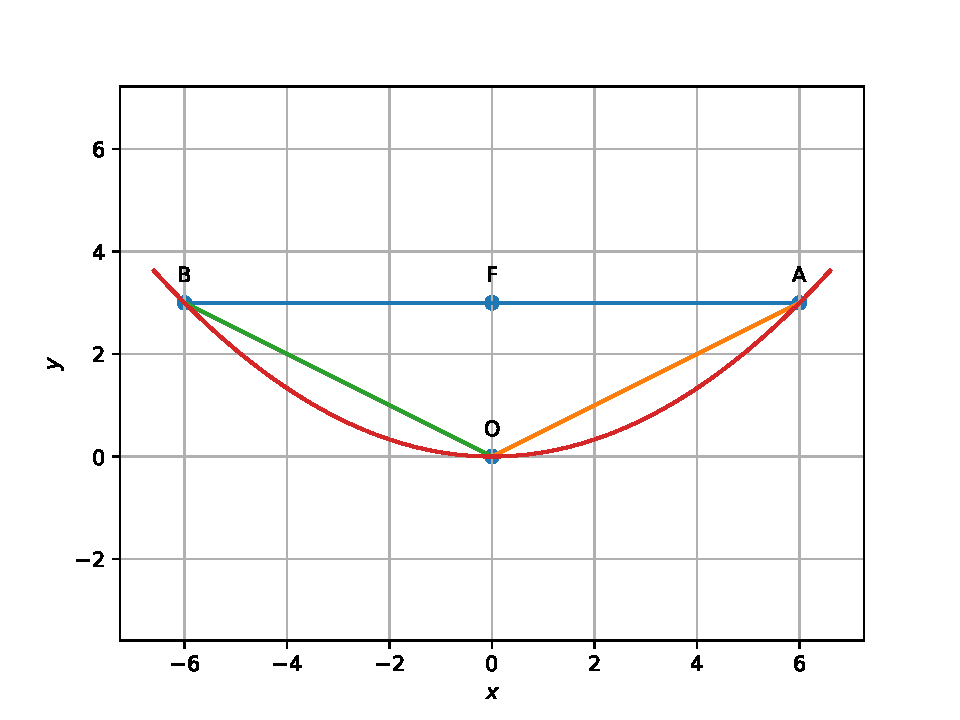
\includegraphics[width=\columnwidth]{chapters/11/11/5/6/figs/fig1.pdf}
		\caption{}
		\label{fig:11/11/5/6}
  	\end{figure}
\iffalse
}

\section*{\large Solution}

\begin{figure}[h]
\centering
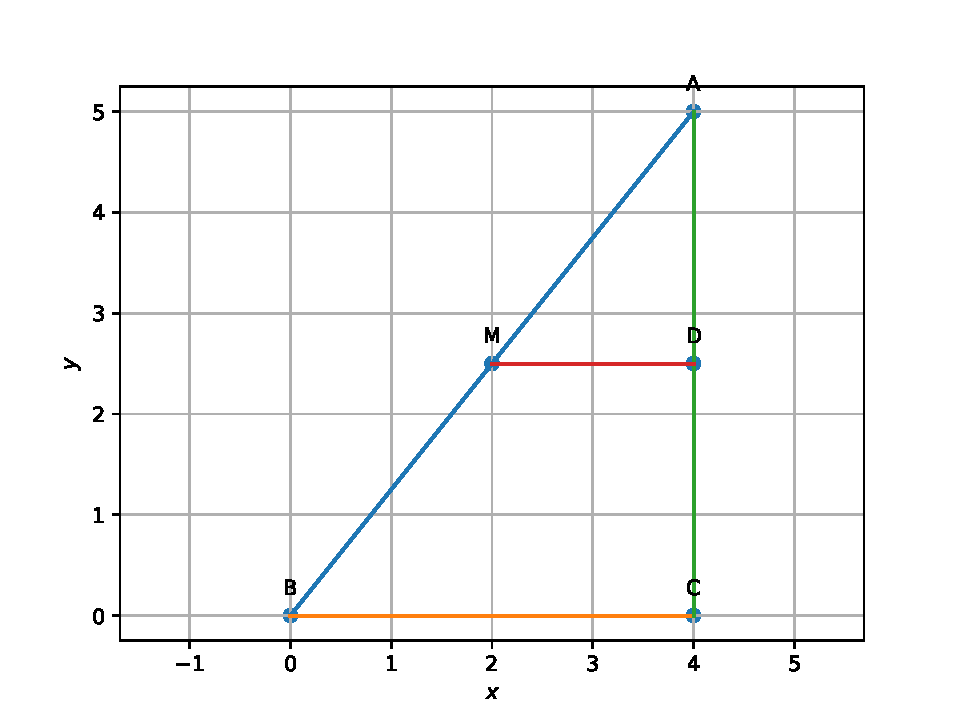
\includegraphics[width=1\columnwidth]{figs/fig1.pdf}
\caption{Triangle formed by vertex and ends of latus rectum of parabola $x^2 = 12y$}
\label{fig:parabola}
\end{figure}

The given equation of parabola $x^2 = 12y$ can be written in the general quadratic form as
\begin{align}
    \label{eq:conic_quad_form}
    \vec{x}^{\top}\vec{V}\vec{x}+2\vec{u}^{\top}\vec{x}+f=0
    \end{align}
where
\begin{align}
	\label{eq:V_matrix}
	\vec{V} &= \myvec{1 & 0\\0 & 0},
	\\
	\label{eq:u_vector}
	\vec{u} &= \myvec{0\\-6},
	\\
	\label{eq:f_value}
	f &= 0
	%\\
\end{align}

The parabola in (\ref{eq:conic_quad_form}) can be expressed in standard form (center/vertex at origin, major-axis - $x$ axis) as
\begin{align}
	\label{eq:conic_simp_parab}
	\vec{y}^{\top}\vec{D}\vec{y} &=  -2\eta\vec{e}_1^{\top}\vec{y}   & \abs{V} &= 0
	\end{align}
 where
\begin{align}
	\label{eq:conic_affine}
	\vec{x} = \vec{P}\vec{y}+\vec{c} \quad \text{(Affine Transformation)}
\end{align}
\begin{align}
	\label{eq:conic_parmas_eig_def}
	\vec{P}^{\top}\vec{V}\vec{P} &= \vec{D}. \quad \text{(Eigenvalue Decomposition)}
	\\
	\label{eq:eigevalV}
	\vec{D} &= \myvec{\lambda_1 & 0\\ 0 & \lambda_2}, 
	\\
	\vec{P} &= \myvec{\vec{p}_1 & \vec{p}_2}, \quad \vec{P}^{\top}=\vec{P}^{-1},
	\label{eq:eigevecP}
	\\
	\label{eq:eta}
	\eta &=\vec{u}^{\top}\vec{p}_1
	\\
	\vec{e}_1 &=\myvec{1 \\ 0}
	\end{align}

To find $\vec{c}$ which is the center of the parabola in (\ref{eq:conic_quad_form}), substitute (\ref{eq:conic_affine}) in (\ref{eq:conic_quad_form})
\begin{multline}
\brak{\vec{P}\vec{y}+\vec{c}}^T\vec{V}\brak{\vec{P}\vec{y}+\vec{c}}+2\vec{u}^T\brak{\vec{P}\vec{y}+\vec{c}} + f = 0, 
\end{multline}
yielding 
\begin{multline}
\vec{y}^T\vec{P}^T\vec{V}\vec{P}\vec{y}+2\brak{\vec{V}\vec{c}+\vec{u}}^T\vec{P}\vec{y} +  \vec{c}^T\vec{V}\vec{c} 
\\
+2\vec{u}^T\vec{c} + f= 0
\label{eq:conic_simp_one}
\end{multline}
%
From \eqref{eq:conic_simp_one} and \eqref{eq:conic_parmas_eig_def},
\begin{multline}
\vec{y}^T\vec{D}\vec{y}+2\brak{\vec{V}\vec{c}+\vec{u}}^T\vec{P}\vec{y} +  \vec{c}^T\brak{\vec{V}\vec{c} + \vec{u}}
\\
+ \vec{u}^T\vec{c} + f= 0
\label{eq:conic_simp}
\end{multline}
For a parabola $\abs{\vec{V}} = 0, \lambda_1 = 0$ and
\begin{align}
\vec{V}\vec{p}_1 = 0, 
\vec{V}\vec{p}_2 = \lambda_2\vec{p}_2.
\label{eq:conic_parab_eig_prop} 
\end{align}
where $\vec{p}_1,\vec{p}_2$ are the eigenvectors of $\vec{V}$ such that  \eqref{eq:conic_parmas_eig_def}
%
\begin{align}
\vec{P} = \myvec{\vec{p}_1 & \vec{p}_2},
\label{eq:eig_matrix}
\end{align}
Substituting \eqref{eq:eig_matrix}
in \eqref{eq:conic_simp},
\begin{multline}
	\vec{y}^T\vec{D}\vec{y}+2\brak{\vec{c}^T\vec{V}+\vec{u}^T}\myvec{\vec{p}_1 & \vec{p}_2}\vec{y}
\\
+  \vec{c}^T\brak{\vec{V}\vec{c} + \vec{u}}+ \vec{u}^T\vec{c} + f= 0
\\
\implies \vec{y}^T\vec{D}\vec{y}
\\
+2\myvec{\brak{\vec{c}^T\vec{V}+\vec{u}^T}\vec{p}_1  \brak{\vec{c}^T\vec{V}+\vec{u}^T}\vec{p}_2}\vec{y}
\\
+  \vec{c}^T\brak{\vec{V}\vec{c} + \vec{u}}+ \vec{u}^T\vec{c} + f= 0
\\
\implies \vec{y}^T\vec{D}\vec{y}
\\
+2\myvec{\vec{u}^T\vec{p}_1 & \brak{\lambda_2\vec{c}^T+\vec{u}^T}\vec{p}_2}\vec{y}
\\
+  \vec{c}^T\brak{\vec{V}\vec{c} + \vec{u}}+ \vec{u}^T\vec{c} + f= 0
\text{ from } \eqref{eq:conic_parab_eig_prop}     \nonumber \\
\\
\implies \lambda_2y_2^2+2\brak{\vec{u}^T\vec{p}_1}y_1+  2y_2\brak{\lambda_2\vec{c}+\vec{u}}^T\vec{p}_2
\\
+  \vec{c}^T\brak{\vec{V}\vec{c} + \vec{u}}+ \vec{u}^T\vec{c} + f= 0
\label{eq:conic_parab_foc_len_temp} 
\end{multline}
which is the equation of a parabola. 
Thus, \eqref{eq:conic_parab_foc_len_temp} 
can be expressed as \eqref{eq:conic_simp_parab} by choosing
\begin{align}
%\label{eq:eta}
\eta = \vec{u}^T\vec{p}_1
\end{align}
and $\vec{c}$ in \eqref{eq:conic_simp} such that
\begin{align}
\label{eq:conic_parab_one}
\vec{P}^{T}\brak{\vec{V}\vec{c}+\vec{u}} &= \eta\myvec{1\\0}
\\
\vec{c}^T\brak{\vec{V}\vec{c} + \vec{u}}+ \vec{u}^T\vec{c} + f&= 0
\label{eq:conic_parab_two}
\end{align}
Multiplying \eqref{eq:conic_parab_one} by $\vec{P}$ yields
\begin{align}
\label{eq:conic_parab_one_eig}
\brak{\vec{V}\vec{c}+\vec{u}} &= \eta\vec{p}_1,
\end{align}
which, upon substituting in \eqref{eq:conic_parab_two}
results in 
\begin{align}
\eta\vec{c}^T\vec{p}_1 + \vec{u}^T\vec{c} + f&= 0
\label{eq:conic_parab_two_eig}
\end{align}
\eqref{eq:conic_parab_one_eig} and \eqref{eq:conic_parab_two_eig} can be clubbed together to obtain \eqref{eq:conic_parab_c}.
\begin{align}
    \myvec{ \vec{u}^{\top}+\eta\vec{p}_1^{\top} \\ \vec{V}}\vec{c} &= \myvec{-f \\ \eta\vec{p}_1-\vec{u}}  &\abs{V} &= 0
    \label{eq:conic_parab_c}
    \end{align}
Substituting appropriate values from \eqref{eq:V_matrix}, \eqref{eq:u_vector}, \eqref{eq:f_value}, \eqref{eq:eigevecP}, and \eqref{eq:eta} into \eqref{eq:conic_parab_c}, the below matrix equation is obtained
\begin{align}
	\label{eq:vertex_system}
	\myvec{0&-12\\1& 0\\0& 0}\vec{c} = \myvec{0 \\0 \\0}\\
\end{align}
The augmented matrix for \eqref{eq:vertex_system} can be expressed as
\begin{align}
	\label{eq:vertex_solv1}
	\myvec{0&-12&\vrule&0\\1&0&\vrule&0\\0&0&\vrule&0}\\ 	
	\label{eq:vertex_solv2}
	\xleftrightarrow[]{R_1 \leftrightarrow R_2}\myvec{1&0&\vrule&0\\0&-12&\vrule&0\\0&0&\vrule&0}\\
	\label{eq:vertex_solv3}
	\xleftrightarrow[]{-\frac{R_2}{12} \leftarrow R_2}\myvec{1&0&\vrule&0\\0&1&\vrule&0\\0&0&\vrule&0}\\
	\label{eq:vertex_solv4}
	\implies\vec{c} = \myvec{0\\0}
\end{align}

From \eqref{eq:V_matrix}
  \begin{multline}
    \vec{V}^{\top} \vec{V}=\brak{\norm{\vec{n}}^2\vec{I}-e^2\vec{n}\vec{n}^{\top}}^{\top}
	  \\
	  \brak{\norm{\vec{n}}^2\vec{I}-e^2\vec{n}\vec{n}^{\top}}
    \\
    \implies \vec{V}^{2} = \norm{\vec{n}}^4\vec{I}+e^4\vec{n}\vec{n}^{\top}\vec{n}\vec{n}^{\top}
	  \\
	  -2e^2\norm{\vec{n}}^2\vec{n}\vec{n}^{\top}
    \\
    = \norm{\vec{n}}^4\vec{I} + e^4\norm{\vec{n}}^2\vec{n}\vec{n}^{\top}
	%  \\
	  - 2e^2\norm{\vec{n}}^2\vec{n}\vec{n}^{\top}
    \\
    = \norm{\vec{n}}^4\vec{I} + e^2\brak{e^2 - 2}\norm{\vec{n}}^2\vec{n}\vec{n}^{\top}
    \\
    = \norm{\vec{n}}^4\vec{I} + \brak{e^2 - 2}\norm{\vec{n}}^2\brak{\norm{\vec{n}}^2\vec{I}- \vec{V}}
    \end{multline}
%    
which can be expressed as
\begin{align}
  \vec{V}^{2} + \brak{e^2 - 2}\norm{\vec{n}}^2\vec{V} - \brak{e^2 - 1}\norm{\vec{n}}^4\vec{I}=0
  \label{eq:conic_quad_form_e_cayley}
\end{align}
Using the Cayley-Hamilton theorem, \eqref{eq:conic_quad_form_e_cayley} results in the characteristic equation, 
\begin{align}
  \lambda^{2} - \brak{2-e^2}\norm{\vec{n}}^2\lambda + \brak{1-e^2 }\norm{\vec{n}}^4=0
\end{align}
which can be expressed as
\begin{multline}
\brak{\frac{\lambda}{\norm{\vec{n}}^2}}^2 - \brak{2-e^2 }\brak{\frac{\lambda}{\norm{\vec{n}}^2}} + \brak{1-e^2 } = 0
\end{multline}
\begin{align}
  \implies \frac{\lambda}{\norm{\vec{n}}^2} = 1-e^2, 1
  \\
  \text{or, }\lambda_2 = \norm{\vec{n}}^2, \lambda_1 = \brak{1-e^2}\lambda_2 
  \label{eq:conic_quad_form_lam_cayley}
\end{align}
From   \eqref{eq:conic_quad_form_lam_cayley}, the eccentricity of \eqref{eq:conic_quad_form} is given by 
\begin{align}
	e &= \sqrt{1-\frac{\lambda_1}{\lambda_2}} 
	\label{eq:conic_quad_form_e}.   
\end{align}
%
% By inspection, we find that 
% \begin{align}
%   \frac{\lambda}}{\norm{\vec{n}}^2} = 1
%   \label{eq:conic_quad_form_lam2_cayley}
% \end{align}
%satisfies \eqref{eq:conic_quad_form_lam_cayley}.
Multiplying both sides of    \eqref{eq:V_matrix} by $\vec{n}$,
\begin{align}
\vec{V} \vec{n}&=\norm{\vec{n}}^2\vec{n}-e^2\vec{n}\vec{n}^{\top}\vec{n} 
\\
&=\norm{\vec{n}}^2\brak{1-e^2}\vec{n} 
 \\
% &=\frac{\lambda_1}{\lambda_2}\norm{\vec{n}}^2\vec{n} 
% \end{align}
% upon substituting from \eqref{eq:conic_quad_form_e}  and simplifying.  From the above, it is obvious that $\vec{n}$ is an eigenvector
% of $\vec{V}$.  Choosing 
% \begin{align}
%   \lambda_2 = \norm{\vec{n}}^2,
%   \label{eq:eigevecn_lam2}
% \end{align}  
% we obtain 
% \begin{align}
  &=\lambda_1 \vec{n} 
  \label{eq:eigevecn}
\end{align}  
from \eqref{eq:conic_quad_form_lam_cayley}
Thus,  $\lambda_1$ is the corresponding eigenvalue for $\vec{n}$.  From       \eqref{eq:eigevecP},   \eqref{eq:conic_quad_form_lam_cayley} and \eqref{eq:eigevecn}, 
\begin{align}
   \vec{n}&= \norm{\vec{n}}\vec{p}_1  = \sqrt{\lambda_2}\vec{p}_1 
\end{align}  
From \eqref{eq:u_vector} and \eqref{eq:conic_quad_form_lam_cayley},
\begin{align}
%   \label{eq:conic_quad_form_v}
% \vec{V} &=\norm{\vec{n}}^2\vec{I}-e^2\vec{n}\vec{n}^{\top}, 
% \\
%\label{eq:conic_quad_form_u}
\label{eq:focus_coord}
\vec{F}  &= \frac{ce^2\vec{n}-\vec{u}}{\lambda_2}
 \\
 \implies \norm{\vec{F}}^2  &= \frac{\brak{ce^2\vec{n}-\vec{u}}^{\top}\brak{ce^2\vec{n}-\vec{u}}}{\lambda_2^2}
 \\
 \implies \lambda_2^2\norm{\vec{F}}^2  &= c^2e^4\lambda_2-2ce^2\vec{u}^{\top}\vec{n}+\norm{\vec{u}}^2
 \label{eq:conic_quad_form_u_temp}
% f &= \norm{\vec{n}}^2\norm{\vec{F}}^2-c^2e^2
% %\\
    \end{align}
    Also, \eqref{eq:f_value} can be expressed as
    \begin{align}
    \lambda_2\norm{\vec{F}}^2 &= f+c^2e^2
    \label{eq:conic_quad_form_f_temp}
\end{align}
From  \eqref{eq:conic_quad_form_u_temp} and     \eqref{eq:conic_quad_form_f_temp},
\begin{align}
c^2e^4\lambda_2-2ce^2\vec{u}^{\top}\vec{n}+\norm{\vec{u}}^2 = \lambda_2\brak{f+c^2e^2}
\end{align}
\begin{multline}
\implies \lambda_2e^2\brak{e^2-1}c^2-2ce^2\vec{u}^{\top}\vec{n}
	\\
	+\norm{\vec{u}}^2 - \lambda_2 f = 0
\end{multline}
yielding
\begin{align}
c &= 
  \begin{cases}
    \frac{e\vec{u}^{\top}\vec{n} \pm \sqrt{e^2\brak{\vec{u}^{\top}\vec{n}}^2-\lambda_2\brak{e^2-1}\brak{\norm{\vec{u}}^2 - \lambda_2 f}}}{\lambda_2e\brak{e^2-1}} & e \ne 1
    \\
    \frac{\norm{\vec{u}}^2 - \lambda_2 f   }{2e^2\vec{u}^{\top}\vec{n}} & e = 1
  \end{cases}
  \label{eq:conic_quad_form_F}.
\end{align}

The points of intersection of the line 
\begin{align}
	L: \quad \vec{x} = \vec{q} + \mu \vec{m} \quad \mu \in \mathbf{R}
\label{eq:conic_tangent}
\end{align}
with the conic section in \eqref{eq:conic_quad_form} are given by
\begin{align}
\vec{x}_i = \vec{q} + \mu_i \vec{m}
\label{eq:conic_tangent_pts}
\end{align}
%
where
{\tiny
\begin{multline}
\mu_i = \frac{1}
{
\vec{m}^T\vec{V}\vec{m}
}
\lbrak{-\vec{m}^T\brak{\vec{V}\vec{q}+\vec{u}}}
\\
\pm
\rbrak{\sqrt{
\sbrak{
\vec{m}^T\brak{\vec{V}\vec{q}+\vec{u}}
}^2
-
\brak
{
\vec{q}^T\vec{V}\vec{q} + 2\vec{u}^T\vec{q} +f
}
\brak{\vec{m}^T\vec{V}\vec{m}}
}
}
\label{eq:tangent_roots}
\end{multline}
}
\\
Substituting \eqref{eq:conic_tangent}
in \eqref{eq:conic_quad_form}, 
\begin{align}
\brak{\vec{q} + \mu \vec{m}}^T\vec{V}\brak{\vec{q} + \mu \vec{m}}  
\\
+ 2 \vec{u}^T\brak{\vec{q} + \mu \vec{m}}+f &= 0
\\
\implies \mu^2\vec{m}^T\vec{V}\vec{m} + 2 \mu\vec{m}^T\brak{\vec{V}\vec{q}+\vec{u}} 
\\
+ \vec{q}^T\vec{V}\vec{q} + 2\vec{u}^T\vec{q} +f &= 0
\label{eq:conic_intercept}
\end{align}
Solving the above quadratic in \eqref{eq:conic_intercept}
yields \eqref{eq:tangent_roots}.

The area of a triangle whose vertices are $\vec{A}, \vec{B}$ and $\vec{O}$ is given by
\begin{align}
	ar(AOB) = \frac{1}{2}\norm{(\vec{A-O})\times(\vec{B-O})}
	\label{eq:tri_area}
\end{align}

\section*{\large Construction}
The input parameters are $\vec{V}$ from \eqref{eq:V_matrix}, $\vec{u}$ from \eqref{eq:u_vector} and $f$ from \eqref{eq:f_value}\\\\
{
\setlength\extrarowheight{5pt}
\begin{tabular}{|c|c|c|}
	\hline
	\textbf{Symbol}&\textbf{Value}&\textbf{Description}\\
	\hline
	$\vec{P}$&\myvec{0&1\\1&0}&eigenvectors of $\vec{V}$\\[5pt]
	\hline
	$\vec{O}$&$\myvec{0\\0}$&center of parabola\\
	\hline
	$\eta$&$\vec{u}^{\top}\vec{p}_1 = -6$&from \eqref{eq:eta}\\[5pt]
	\hline
	$\lambda_2$&$\vec{e}_2^{\top}D\vec{e}_2 = 1$&from \eqref{eq:eigevalV}\\[5pt]
	\hline
	$\vec{n}$&$\sqrt{\lambda_2}\vec{p_1} = \myvec{0\\1}$&normal to directrix\\[5pt]
	\hline
	$c$&from \eqref{eq:conic_quad_form_F}&$\vec{n}^\top\vec{x} = c$\\
	\hline
	$\vec{F}$&$\myvec{0\\3}$&focus from \eqref{eq:focus_coord}\\[5pt]
	\hline
	$\vec{m}$&$\myvec{1\\0}$&latus rectum direction vector\\[5pt]
	\hline
	$\myvec{\vec{A} \\ \vec{B}}$&$\myvec{\vec{F} + \mu_1\vec{m} \\ \vec{F} + \mu_2\vec{m}}$&$\mu_1, \mu_2$ from \eqref{eq:tangent_roots}\\[5pt]
	\hline
	ar(AOB)&18 sq units&from \eqref{eq:tri_area}\\
	\hline
\end{tabular}
}

\end{document}
\fi

\item A man running a racecourse notes that the sum of the distances from the two flag posts from him is always 10 m and the distance between the flag posts is 8 m. Find the equation of the posts traced by the man. 
\label{chapters/11/11/5/7}
\iffalse
\documentclass[12pt]{article}
\usepackage{graphicx}
\usepackage[none]{hyphenat}
\usepackage{graphicx}
\usepackage{listings}
\usepackage[english]{babel}
\usepackage{graphicx}
\usepackage{caption} 
\usepackage{booktabs}
\usepackage{array}
\usepackage{amssymb} % for \because
\usepackage{amsmath}   % for having text in math mode
\usepackage{extarrows} % for Row operations arrows
\usepackage{listings}
\lstset{
  frame=single,
  breaklines=true
}
\usepackage{hyperref}
  
%Following 2 lines were added to remove the blank page at the beginning
\usepackage{atbegshi}% http://ctan.org/pkg/atbegshi
\AtBeginDocument{\AtBeginShipoutNext{\AtBeginShipoutDiscard}}


%New macro definitions
\newcommand{\mydet}[1]{\ensuremath{\begin{vmatrix}#1\end{vmatrix}}}
\providecommand{\brak}[1]{\ensuremath{\left(#1\right)}}
\providecommand{\norm}[1]{\left\lVert#1\right\rVert}
\providecommand{\abs}[1]{\left\vert#1\right\vert}
\newcommand{\solution}{\noindent \textbf{Solution: }}
\newcommand{\myvec}[1]{\ensuremath{\begin{pmatrix}#1\end{pmatrix}}}
\let\vec\mathbf


\begin{document}

\begin{center}
\title{\textbf{Conic Sections - Ellipse}}
\date{\vspace{-5ex}} %Not to print date automatically
\maketitle
\end{center}
\setcounter{page}{1}

\section{11$^{th}$ Maths - Chapter 11}
This is Problem-7 from Exercise 11.5
\begin{enumerate}

\solution 
\fi
The conic section for the given problem is an ellipse. Let $\vec{O}\myvec{0 \\ 0}$ be the centre of the Ellipse. Then, the focii are given by 
\begin{align}
    \label{eq:chapters/11/11/5/7/ellipseEq1}
	\vec{F_1} = \myvec{ 4 \\ 0} \\
	\vec{F_2} = \myvec{ -4 \\ 0} 
\end{align}
The sum of the distances from two focii to the point on the locus of the ellipse is equal to $10m$. Let $\vec{P}\myvec{p \\ 0 }$ and $\vec{Q}\myvec{-q \\ 0}$ be the vertices of the ellipse. Then
\begin{align}
	\norm{\vec{P}-\vec{F_1}} + \norm{\vec{P}-\vec{F_2}} = 10 \\
         \brak{p-4} + \brak{p+4} = 10 \\
	 2p = 10 \\
	 p = 5  \\
	 \therefore \vec{P} = \myvec{5 \\ 0}
\end{align}
Similarly
\begin{align}
	\norm{\vec{Q}-\vec{F_1}} + \norm{\vec{Q}-\vec{F_2}} = 10 \\
         \brak{q-4} + \brak{q+4} = 10 \\
	 2q = 10 \\
	 q = 5 \\
	 \therefore \vec{Q} = \myvec{-5 \\ 0}
\end{align}
We know that the Vertex of a standard ellipse is given by
\begin{align}
	\vec{P} &=  \myvec{\sqrt{\abs{\frac{f_0}{\lambda_1}}} \\ 0} \\
	\myvec{5 \\ 0} &=  \myvec{\sqrt{\abs{\frac{f_0}{\lambda_1}}} \\ 0} \\
	\frac{f_0}{\lambda_1} &= 25 \\
	\label{eq:chapters/11/11/5/7/eqV}
	f_0 &= 25\lambda_1 
\end{align}
We know that the Focii for standard Ellipse are given as
\begin{align}
	\label{eq:chapters/11/11/5/7/eqV1}
	\vec{F} &= \pm e\sqrt{\frac{\abs{f_0}}{\lambda_2\brak{1-e^2}}}\vec{e}_1
\end{align}
Substituting values of $\vec{F_1}$ from \eqref{eq:chapters/11/11/5/7/ellipseEq1} and $f_0$ from \eqref{eq:chapters/11/11/5/7/eqV}
\begin{align}
	   \label{eq:chapters/11/11/5/7/eqV2}
	   \eqref{eq:chapters/11/11/5/7/eqV1} \implies \myvec{4 \\0}  &=e\sqrt{\frac{25\lambda_1}{\lambda_2\brak{1-e^2}}}\vec{e}_1
\end{align}
We know that 
\begin{align}
	1-e^2 = \frac{\lambda_1}{\lambda_2} \\
	\eqref{eq:chapters/11/11/5/7/eqV2} \implies  4 &= 5e \\
        e &= \frac{4}{5} \\
	\therefore \frac{\lambda_1}{\lambda_2} &= 1 - \brak{\frac{4}{5}}^2 \\
	&= \frac{9}{25} \\
	\vec{n} &= \sqrt{\frac{\lambda_2}{f_0}}\vec{e}_1\\
	 &= \sqrt{\frac{\lambda_2}{25\lambda_1}}\vec{e}_1\\
	 &= \frac{1}{5} \times \frac{5}{3}\vec{e}_1\\
	 &= \frac{1}{3}\vec{e}_1 \\
	 c &= \frac{1}{e\sqrt{1-e^2}} = \frac{25}{12}
\end{align}
For the standard ellipse, $f$ is given as 
\begin{align}
	\label{eq:chapters/11/11/5/7/eqV3}
	f &= \norm{\vec{n}}^2 \norm{\vec{F}}^2 - c^2 e^2 \\
	&= \brak{\frac{1}{3}}^216 - \frac{25}{9} \\
	&= -1 \\
	f_0 &= -f = 1 \\
	\lambda_1 &= \frac{f_0}{25} = \frac{1}{25}\\
	\lambda_2 &= \frac{25\lambda_1}{9} = \frac{1}{9} \\
	\therefore \vec{V} &= \myvec{\lambda_1 & 0 \\ 0 & \lambda_2} = \myvec{\frac{1}{25} & 0 \\ 0 & \frac{1}{9}}
\end{align}
For a standard ellipse, $\vec{u}=0$. 

The generic equation of conic section is given as
\begin{align}
	\label{eq:chapters/11/11/5/7/ellipseEq2}
	g\brak{\vec{x}} &= \vec{x}^T\vec{V}\vec{x} + 2\vec{u}^T\vec{x} + f = 0 \\ 
	&= \vec{x}^T\myvec{\frac{1}{25} & 0 \\ 0 & \frac{1}{9}}\vec{x}- 1  = 0 
\end{align}
The relevant diagram is shown in Figure \ref{fig:chapters/11/11/5/7/Fig1}
\begin{figure}[!h]
	\begin{center}
		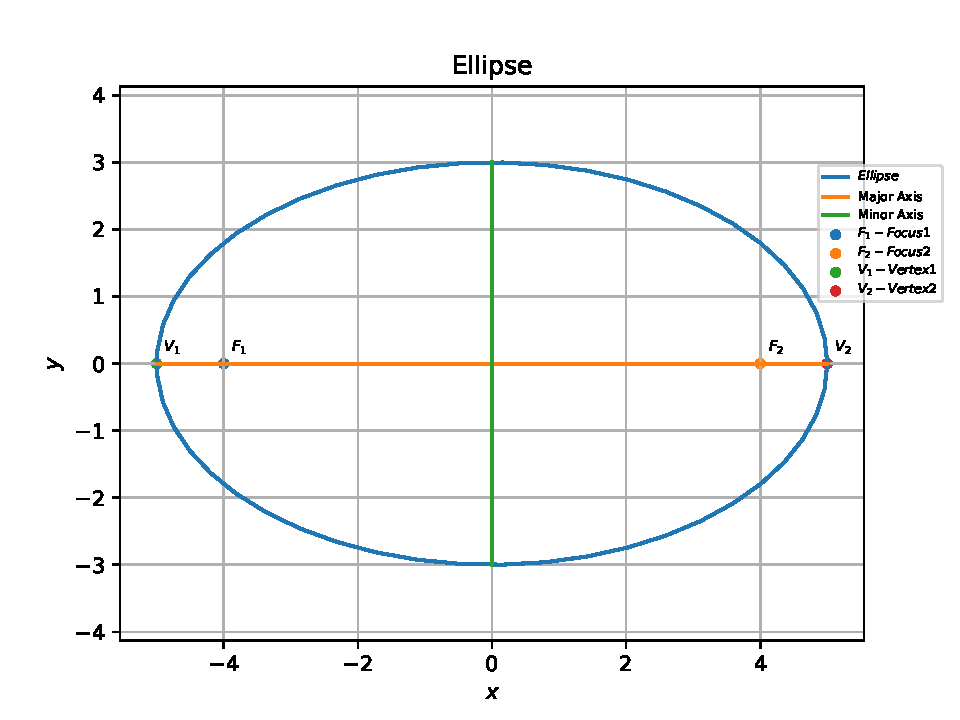
\includegraphics[width=\columnwidth]{chapters/11/11/5/7/figs/problem7.pdf}
	\end{center}
\caption{}
\label{fig:chapters/11/11/5/7/Fig1}
\end{figure}

\item 
\label{chapters/11/11/5/8}
\iffalse
\documentclass[journal,10pt,twocolumn]{article}
\usepackage{graphicx}
\usepackage[margin=0.5in]{geometry}
\usepackage[cmex10]{amsmath}
\usepackage{array}
\usepackage{booktabs}
\usepackage{mathtools}
\usepackage{amssymb}
\title{\textbf{Conics Assignment}}
\author{Alavala Chinnapa Reddy}
\date{September 2022}
\providecommand{\norm}[1]{\left\lVert#1\right\rVert}
\providecommand{\abs}[1]{\left\vert#1\right\vert}
\let\vec\mathbf
\newcommand{\myvec}[1]{\ensuremath{\begin{pmatrix}#1\end{pmatrix}}}
\newcommand{\mydet}[1]{\ensuremath{\begin{vmatrix}#1\end{vmatrix}}}
\providecommand{\brak}[1]{\ensuremath{\left(#1\right)}}
\providecommand{\lbrak}[1]{\ensuremath{\left(#1\right.}}
\providecommand{\rbrak}[1]{\ensuremath{\left.#1\right)}}
\providecommand{\sbrak}[1]{\ensuremath{{}\left[#1\right]}}
\begin{document}

\maketitle
\paragraph{\textit{Problem Statement} -
\fi
An equilateral triangle is inscribed in the parabola $y^{2} = 4ax$,where one vertex is at the vertex of the parabola. Find the length of the side of the triangle.
	\begin{figure}[!ht]
		\centering
 \includegraphics[width=\columnwidth]{chapters/11/11/5/8/figs/co.pdf}
		\caption{}
		\label{fig:11/11/5/8}
  	\end{figure}
\\
\solution
\iffalse
} \vspace{5mm}
\section*{\large Solution}


Given, the axis of parabola is horizotal.
\\ Given,one vertex of $\triangle$OAB is at vertex of parabola.

\begin{figure}[h]
\includegraphics[width=0.8\columnwidth]{figs/co.pdf}
\end{figure}
\begin{equation}
  \label{eq:std_parabola}
  \textbf{x}^T\textbf{V}\textbf{x}+2\textbf{u}^T\textbf{x}+f=0
\end{equation}
where,
\begin{eqnarray}
	\vec{O}=\myvec{0\\0}
\end{eqnarray}	
Equation Parabola is $y^2=4ax$\\
From $\triangle$OAB
\begin{eqnarray}
	\norm{\vec{A}}=\norm{\vec{B}}=\norm{\vec{A-B}}\\
	\norm{\vec{A}}^2=\norm{\vec{B}}^2=\norm{\vec{A-B}}^2\\
	\norm{\vec{A}}^2+\norm{\vec{B}}^2-2\vec{A}^T\vec{B}=\norm{\vec{A}}^2=\norm{\vec{B}}^2\\
	\frac{\vec{A}^T\vec{B}}{\norm{\vec{A}}^2}=\frac{\vec{A}^T\vec{B}}{\norm{\vec{B}^2}}=\frac{1}{2}
\end{eqnarray}
$\triangle$OAB is a equilateral triangle\\
$\alpha$=$60^{0}$\\
The side length of equilateral triangle,OA=OB=AB=r\\
Let
\begin{eqnarray}
	\vec{A}=\myvec{r\cos{\theta_1}\\r\sin{\theta_1}}\\
	\vec{B}=\myvec{r\cos{\theta_2}\\r\sin{\theta_2}}
\end{eqnarray}
\begin{eqnarray}
	\vec{A}^T\vec{B}=\frac{\norm{\vec{A}}^2}{2}\\
	r^2\cos{(\theta_1-\theta_2)}=\frac{r^2}{2}\\
	\theta_1-\theta_2=\cos{^{-1}\frac{1}{2}}
\end{eqnarray}
Given $\vec{A}$ satisfy the eq1
\begin{eqnarray}
	\vec{A}^T\vec{V}\vec{A}+2\vec{u}^T\vec{A}+f=0\\
	\vec{A}^T\vec{V}\vec{A}+2\vec{u}^T\vec{A}=0
\end{eqnarray}
\begin{equation}
	\myvec{r\cos{\theta_1}&r\sin{\theta_1}}\myvec{0&0\\0&1}\myvec{r\cos{\theta_1}\\r\sin{\theta_1}}+2\myvec{-2a&0}\myvec{r\cos{\theta_1}\\r\sin{\theta_1}}=0
\end{equation}
\begin{equation}
	\myvec{r\cos{\theta_1}&r\sin{\theta_1}}\myvec{0\\r\sin{\theta_1}}+2(-2ar\cos{\theta_1})=0
\end{equation}
\begin{eqnarray}
	r^2\sin{^2\theta_1}=4ar\cos{\theta_1}\\
	r=\frac{4a\cos{\theta_1}}{\sin{^2\theta_1}}
\end{eqnarray}
Similarly $\vec{B}$ satisfy the eq1
\begin{equation}
	r=\frac{4a\cos{\theta_2}}{\sin{^2\theta_2}}
\end{equation}
Form eq17 and eq18\\
Yeilding
\begin{eqnarray}
	\cos{(\theta_1+\theta_2)}=1\\
	\theta_1+\theta_2=\cos{^{-1}1}
\end{eqnarray}
Add eq11 and eq20\\
\begin{equation}
	\theta_1=\frac{\cos{^{-1}\frac{1}{2}+\cos{^{-1}1}}}{2}
\end{equation}
Subtract eq20 from eq11
\begin{equation}   
\theta_2=\frac{-\cos{^{-1}\frac{1}{2}+\cos{^{-1}1}}}{2}        
\end{equation}
 \section*{\large Construction} The input parameters are V,u,f \\
 $\vec{V}=\myvec{0&0\\0&1},\vec{u}=\myvec{-2a\\0},f=0$\\
\setlength\extrarowheight{7pt}
\begin{tabular}{|c|c|c|}
  \hline
  \textbf{Symbol}&\textbf{Value}&\textbf{Description}\\
  \hline
	a&1&\\
  \hline
	$\alpha$&$60^{0}$&$\angle{A}=\angle{B}=\angle{O}$\\
	\hline
	r&Solving eq18&OA=OB=AB\\
	\hline
  $\vec{O}$&$\myvec{0\\0}$&center of parabola and Point O\\
  \hline
	$\vec{A}$&$\myvec{r\cos{\theta_1}\\r\sin{\theta_1}}$&Point A\\[8pt]
  \hline
	$\vec{B}$&$\myvec{r\cos{\theta_2}\\r\sin{\theta_2}}$&Point B\\[8pt]  \hline
\end{tabular}
\end{document}
\fi


\end{enumerate}
